\documentclass[12pt, a4paper]{article}

\usepackage[utf8]{inputenc}
\usepackage[spanish]{babel}
\usepackage{titling}
\usepackage[left=2cm,right=2cm,top=2cm,bottom=2cm]{geometry}
\usepackage{enumerate}
\usepackage{amsmath}
\usepackage{graphicx}
\usepackage{caption}

\usepackage{listings}%-para agregar codigo-
\usepackage[usenames,dvipsnames]{color}
\usepackage{color}%------------------------

%---------------------importar codigo desde archivos cpp----------------------------
\lstloadlanguages{C++}
\lstnewenvironment{code}
	{%\lstset{	numbers=none, frame=lines, basicstyle=\small\ttfamily, }%
	 \csname lst@SetFirstLabel\endcsname}
	{\csname lst@SaveFirstLabel\endcsname}
\lstset{% general command to set parameter(s)
	language=C++, basicstyle=\small\ttfamily, keywordstyle=\slshape,
	emph=[1]{tipo,usa}, emphstyle={[1]\sffamily\bfseries},
	morekeywords={tint,forn,forsn},
	basewidth={0.47em,0.40em},
	columns=fixed, fontadjust, resetmargins, xrightmargin=5pt, xleftmargin=15pt,
	flexiblecolumns=false, tabsize=2, breaklines,	breakatwhitespace=false, extendedchars=true,
	numbers=left, numberstyle=\tiny, stepnumber=1, numbersep=9pt,
	frame=l, framesep=3pt,
    basicstyle=\ttfamily,
    keywordstyle=\color{blue}\ttfamily,
    stringstyle=\color{magenta}\ttfamily,
    commentstyle=\color{RedOrange}\ttfamily,
    morecomment=[l][\color{OliveGreen}]{\#}
}

\lstdefinestyle{C++}{
	language=C++, basicstyle=\small\ttfamily, keywordstyle=\slshape,
	emph=[1]{tipo,usa,tipo2}, emphstyle={[1]\sffamily\bfseries},
	morekeywords={tint,forn,forsn},
	basewidth={0.47em,0.40em},
	columns=fixed, fontadjust, resetmargins, xrightmargin=5pt, xleftmargin=15pt,
	flexiblecolumns=false, tabsize=2, breaklines,	breakatwhitespace=false, extendedchars=true,
	numbers=left, numberstyle=\tiny, stepnumber=1, numbersep=9pt,
	frame=l, framesep=3pt,
    basicstyle=\ttfamily,
    keywordstyle=\color{blue}\ttfamily,
    stringstyle=\color{magenta}\ttfamily,
    commentstyle=\color{RedOrange}\ttfamily,
    morecomment=[l][\color{OliveGreen}]{\#}
}

\def\nbtitle#1{\begin{Large}\begin{center}\textbf{#1}\end{center}\end{Large}}
\def\nbsection#1{\section{#1}}
\def\nbsubsection#1{\subsection{#1}}
\def\nbcoment#1{\begin{small}\textbf{#1}\end{small}}
\newcommand{\comb}[2]{\left( \begin{array}{c} #1 \\ #2 \end{array}\right)}
\def\complexity#1{\texorpdfstring{$\mathcal{O}(#1)$}{O(#1)}}
 \newcommand\cppfile[2][]{
\lstinputlisting[style=C++,linerange={#1}]{#2}
}
%%------------------------------------------------------------------------------

\newcommand{\subtitulo}[1]{\begin{center}\textbf{#1}\end{center}}

\title{\textbf{Matematicas}}
\author{Wilmer Emiro Castrillón Calderón}

\graphicspath{{../}}
\newcommand*\lstinputpath[1]{\lstset{inputpath=#1}}
\lstinputpath{../}

\begin{document}
	\maketitle
	
	%<*Capitulo>
	
	\section{MCD y MCM}
	\label{matematicas:mcd_y_mcm}
	
	\subtitulo{MCD (Máximo común divisor)}
	
	El máximo común divisor de un conjunto de dos o mas números enteros es el máximo número entero el cual divide a  
	todos los números del conjunto sin dejar residuo, por ejemplo el máximo común divisor de $35$ y $15$ es $5$ porque  
	es el máximo entero el cual los puede dividir a ambos. Como abreviatura se utiliza MCD o en ingles GCD (greatest  
	common divisor).\\
	
	El calculo del MCD de dos números se puede hacer de manera eficiente utilizando el algoritmo de Euclides el cual
	se puede realizar en $O(log(n))$ pasos, antes de explicarlo es necesario tener en cuenta las dos siguientes 
	propiedades de la divisibilidad ($x|y$ significa que $x$ divide a $y$ con residuo $0$).
	
	\begin{equation}
		\label{matematicas:eq:division1}
		x|y \rightarrow x| \alpha y \quad \forall \alpha \in Z
	\end{equation}
	
	\begin{equation}
		\label{matematicas:eq:division2}
		x|y \wedge x|y \pm z \rightarrow x|z
		%x|y \wedge x|z \rightarrow x| \alpha y + \beta z \quad \forall \alpha, \beta \in Z
	\end{equation}
	
	El algoritmo consiste en lo siguiente: dado dos números $a$ y $b$ se realiza la división entre ambos, obteniendo un
	cociente $q$ y un residuo $r$, entonces $a = b*q_{1} + r_{1}$ con $r_{1} < b$, teniendo en cuenta que el MCD divide 
	a $a$ y $b$ entonces también divide $b*q_{1}$ (propiedad \ref{matematicas:eq:division1}), y también divide a 
	$r_1$ (propiedad \ref{matematicas:eq:division2}), el proceso se reduce a encontrar el MCD entre $b$ y $r_{1}$ 
	entonces se repite el proceso, $r_{1} = b*q_{2} + r_{2}$ con $r_{2} < r_{1}$, y así sucesivamente hasta llegar a 
	$r_{n} = 0$, lo cual indica que $r_{n-1}$ divide a $r_{n-1}$, $r_{n-2}$, ..., $b$ y $a$, entonces $r_{n-1}$ es el 
	MCD.
	
	\begin{align*}
		a &= b*q_{1} + r_{1} & r_{1} < b\\
		b &= r_{1}*q_{2} + r_{2} & r_{2} < r_{1} \\
		r_{1} &= r_{2}*q_{3} + r_{3} & r_{3} < r_{2} \\
		...\\
		r_{n-1} &= r_{n}*q_{n+1} + 0 & 0 < r_{n} \\
	\end{align*}
	
	Por ejemplo, con $a = 35$ y $b = 15$, $a = b*2 + 5$, $r_{1} = 5$, en el siguiente paso $b = 5*3 + 0$, $r_{2} = 0$, 
	como se ha llegado a un residuo $0$, el algoritmo finaliza y la respuesta es el ultimo residuo diferente de $0$,
	entonces $MCD(35,15) = 5$.\\
	
	\subtitulo{MCM (Mínimo común múltiplo)}
	
	El mínimo común múltiplo de un conjunto de números enteros es el numero entero mas pequeño el cual es múltiplo de
	todos los números del conjunto, por ejemplo el mínimo común múltiplo de $35$ y $15$ es $105$, pues es el menor entero
	tal que $35|105$ y $15|105$. Como abreviatura se usa MCM o en ingles LCM (lowest common multiple).\\
	
	Para calcular el MCM también se puede utilizar el algoritmo de Euclides, pues existe una relación entre el MCD
	y el MCM. entonces $MCM(a*b) = (a*b)/MCD(a,b)$, esta formula es equivalente
	a $a*(b/MCD(a,b))$ como $MCD(a,b) | b$ se puede observar que el resultado sera un entero múltiplo de $a$, de igual
	es equivalente a $b*(a/MCD(a,b))$ y el resultado es un entero múltiplo de $b$, entonces $(a*b)/MCD(a,b)$
	es múltiplo común de $a$ y $b$.\\
	
	Por ejemplo, con $a = 35$ y $b = 15$ el $MCM(a,b) = 35*15/5$ (en el ejemplo anterior se calculo el MCD 
	de $a$ y $b$), entonces el resultado es $105$.
	
	\subtitulo{Implementación}
	
	La implementación del MCD consiste en simplemente aplicar los pasos descritos para el algoritmo de Euclides. La 
	implementación del MCM consiste en aplicar la formula, se recomienda realizar primero la división para evitar un  
	posible overflow al trabajar con números grandes.
	
	\begin{figure}[!htb]
		\minipage{0.5\textwidth}
			\centering
			\cppfile[5-8]{Matematicas/codigos/MCD_y_MCM.cpp}
			MCD
		\endminipage
		\minipage{0.5\textwidth}
			\centering
			\cppfile[10-12]{Matematicas/codigos/MCD_y_MCM.cpp}
			MCM
		\endminipage
	\end{figure}
	
	\section{Criba de Eratóstenes}
	\label{matematicas:criba_de_eratostenes}
	
	La búsqueda de números primos es un problema clásico, las soluciones sencillas se basan en tomar un numero $x$
	y empezar a validar si algún numero en el intervalo $[2, x-1]$ divide a $x$, si ninguno lo divide entonces $x$ es
	un numero primo, esta idea se puede mejorar un poco, se puede validar desde el comienzo si $x$ es un numero par, en
	ese caso $x$ es primo solamente si es igual a $2$, pues el único numero primo par es el $2$, si $x$ es impar se 
	hace la validación si algún numero impar en el intervalo $[3, x-1]$ divide a $x$, existe una propiedad la cual
	indica que el menor factor primo de un numero $x$ es menor a $\sqrt{x}$, entonces nuevamente es posible reducir 
	el intervalo, finalmente un entero positivo $x$ mayor a $1$ es primo si es igual a $2$ o si ningún numero impar
	en el intervalo $[3, \sqrt{x}]$ divide a $x$. Este método tiene complejidad $O(\sqrt{x})$ para cada numero, si 
	se necesita	verificar $n$ números, el proceso se tendría que repetir $n$ veces, por lo tanto si se requiere 
	obtener una lista de números primos se tiene que buscar una mejor solución\\
	
	La criba de Eratóstenes es un algoritmo para encontrar todos los números primos hasta un numero $n$, cosiste de un
	arreglo de números los cuales se irán marcando si son compuestos, si no están marcados entonces son primos,
	inicialmente todos son considerados primos (no están marcados), 
	se comienza tomando el $2$ y se marcan todos los múltiplos de $2$ como números compuestos, después se toma el $3$ 
	y se marcan todos los múltiplos de $3$ como números compuestos, al llegar al $4$ este ya estará marcado entonces el
	$4$ es compuesto, en este caso se omite y se pasa al $5$ el cual no esta marcado, y así sucesivamente, los números
	que no estén marcados son números primos, en la figura \ref{matematicas:criba_de_eratostenes:ejemplo}
	se puede observar un sencillo ejemplo con $n = 17$.\\
	
	\begin{figure}[!htb]
		\centering
		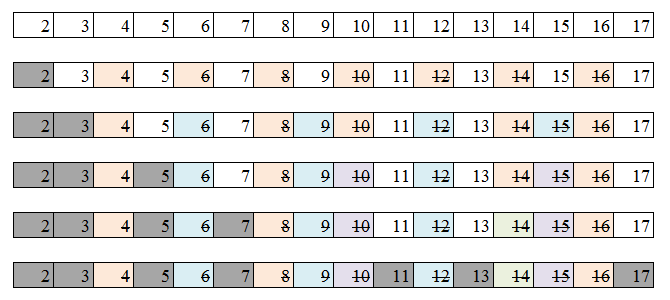
\includegraphics[scale=0.9]{Matematicas/imagenes/criba_de_eratostenes/ejemplo}
		\caption{}
		\label{matematicas:criba_de_eratostenes:ejemplo}
	\end{figure}
	
	La implementación consiste en usar un arreglo de bool inicialmente en true (a excepción del $0$ y $1$ que no son 
	primos), después se recorre el arreglo verificando los números que no estén marcados, para cada numero $i$ no 
	marcado se empieza a marcar los múltiplos de $i$, los múltiplos se pueden empezar a marcar desde $i^2$. Al final
	se obtiene un arreglo el cual permite validar si un $i$ es primo y permite obtener un vector con la lista de 
	números primos hasta $n$, el algoritmo tiene complejidad $O(n*log(log(n)))$.
	
	\cppfile[7-21]{Matematicas/codigos/criba.cpp}
	
	%</Capitulo>
	
\end{document}


